\subsection{Inductive Conformal Prediction (ICP)}


Let $\mathcal{D} = (z_1, \ldots, z_n)$ be a dataset of size $n$. We denote $z_i = (x_i,y_i)$ as a sample of an input and output pair that follows the distribution $\mathcal{P}$, where $i$ is the data index. The input space $\mathbf{X}$ and target space $ \mathbf{Y}$ can be two arbitrary measurable spaces, their Cartesian product $\mathbf{Z} = \mathbf{X} \times \mathbf{Y}$ is the sample space. We begin the algorithm by splitting the dataset into a proper training set $\Dtrain$ with $|\Dtrain| = m$ and a calibration set $\Dcal$ with $|\Dcal| = n-m$. The objective of conformal prediction is produce a \textit{valid} confidence region (Definition \ref{def:validity}).  

\begin{definition}[Validity]
Given a new data pair $(X,Y) \sim  \mathcal{P}$ and a desired coverage rate $1-\alpha \in (0,1)$, region $\Gamma^{1-\alpha}$(x) is \textit{valid} if
\[ \Prob_{(X,Y) \sim \gP} (Y \in \Gamma^{1-\alpha}(X)) \geq 1-\alpha
\]
\label{def:validity} 
\end{definition}


An important component of conformal prediction is the \textit{nonconformity score} $A : \mathbf{Z} \times \mathbf{Z}^m  \rightarrow \mathbb{R}$, a function to capture how well a sample $z$ \textit{conforms} to the proper training set. 
For example, we may choose nonconformity score $A(z, \mathcal{D}_{train})$ to be the L2-loss on the new sample:
\begin{equation}
   A(z, \mathcal{D}_{train}) := \edit{\|} y - \hat{f}(x) \edit{\|}
\end{equation}
where $\hat{f}: \mathbf{X}\longrightarrow \mathbf{Y}$ is a forecasting model trained with the proper training set $\mathcal{D}_{train}$. In the following sections, we refer to the nonconformity score of a sample $z$ given forecasting model $\hat{f}$ as $A(z, \hat{f})$ for simplicity. Let $s_i = A(z_i, \hat{f})$ denote the nonconformity score of a sample $z_i$ and let $s_{cal} = \{A(z_i, \hat{f})\}_{z_i \in \Dcal}$ denote the set of nonconformity scores of all samples in $\Dcal$. We define the empirical $p$-quantile of the set of nonconformity scores $\gS$ as:
\begin{equation}
    Q(p, \gS) := \inf\{s': (\frac{1}{|\gS|} \sum_{s_i \in \gS} \mathbbm{1}_{s_i \leq s'}) \geq p \}
    \label{eq:quantile}
\end{equation}

\begin{definition}[\edit{Exchangeability}]
In a dataset $\{z_1, z_2, \ldots, z_n\}$ of length  $n$, any of its $n$! permutations are equally probable. 
\label{def:exchangability}
\end{definition}

Under the exchangeablility assumption (definition \autoref{def:exchangability}), conformal prediction is theoretically guaranteed to be valid (definition \ref{def:validity}). Let $z_{n+1} = (x_{n+1}, y_{n+1}) \in \mathbf{Z}$ be a new sample, and let $\alpha \in [0,1]$ be a chosen significance level (and $1-\alpha$ the confidence level). Since $D_{cal} \cup \{z_{n+1}\}$ is exchangeable, the probability of $A(z_{n+1})$'s rank among $\{A(z_{i})\}_{z_{i} \in \mathcal{D}_{cal}}$ is uniform. Therefore,
                  
\begin{equation}
\Prob(A(z_{n+1}, \hat{f}) \leq Q(1-\alpha, s_{cal}\cup \{\infty\})) = \frac{ \ceil{|(\mathcal{D}_{cal}| +1)(1-\alpha)}}{|\mathcal{D}_{cal}|+1} \geq 1-\alpha   \label{eq:validityproof}
\end{equation}

The conformal confidence region is constructed as in equation \ref{eq:region}. We say a sample is \textit{covered} if the true value is in the confidence region $y_{n+1} \in \Gamma^{1-\alpha}(x_{n+1})$. Equation \ref{eq:validityproof} means the probability of $y_{n+1}$ being covered is greater than $1-\alpha$, hence the confidence region is valid.
\begin{equation}
    \Gamma^{1-\alpha}(x_{n+1}) := \{ y : A(\edit{z_{n+1}}, \hat{f}) \leq Q(1-\alpha, s_{cal}\cup \{\infty\})\}
    \label{eq:region}
\end{equation}

%(see proposition 4.1 in \cite{vovk2005algorithmic} for full proof).
The procedure introduced above is known as \textit{inductive} or \textit{split} conformal prediction, as it splits the dataset into training and calibration sets to reduce the amount of computation \cite{vovk2005algorithmic,lei2012distribution}. We introduce it as it is commonly used for uncertainty quantification for machine learning models \cite{papadopoulos2008inductive}. Although our method in this paper, CopulaCPTS, is implemented based on inductive CP, it can be easily adjusted for other CP variants.


\subsection{Copula and Its Properties}

In this paper we will model the dependency between time step's uncertainty with copulas. Copula is a concept from statistics that describes the dependency structure in a multivariate distribution. We can use Copulas to capture the joint distribution for multiple future time steps. 
% 1. widely used in economics
% 2. Machine learning for probablisitic time series forecasting, but not related to CP
% 3. used to model dependencies between multitargets (non temporal) by messoudi et al.

This section will briefly introduce its notations and concepts.

\begin{definition}[Copula]
Given a random vector $(X_1,\cdots X_k)$, define the marginal cumulative density function (CDF) as $F_i(x) = P(X_i \leq x)$,  the copula of $(X_1, \cdots X_k)$ is the \edit{joint} CDF of $(U_1,\cdots, U_k) = (F_1(X_1), \cdots, F_k(X_k))$, meaning 
\[ C(u_1,\cdots, u_k)  = P(U_1\leq u_1, \cdots, U_k\leq u_k)\]
Alternatively
\[ C(u_1,\cdots, u_k)  = P(X_1\leq F_1^{-1}(u_1), \cdots, X_k\leq F_t^{-1}(u_k)) \]
\end{definition}

In other words, the Copula function captures the dependency structure between the variable $X$s; we can view an $k$ dimensional copula $C: [0,1]^k \rightarrow [0,1]$ as a CDF with uniform marginals. A fundamental result in the theory of copula is Sklar's theorem. 

\begin{theorem}[Sklar's theorem]
Given a \edit{joint} CDF  as $F(X_1,\cdots, X_k)$ and the marginals $F_i(x)$,  there exists a copula such that 
\[F(x_1,\cdots, x_k) = C(F_1(x_1), \cdots, F_k(x_k))\]
for all $x_i\in [-\infty, \infty]$ and $i =1, \cdots, k$.
\end{theorem}

Sklar's theorem states that for all multivariate distribution functions, there exists a copula function such that the distribution can be expressed using the copula and multiple univariate marginal distributions. To give an example, when all the $X_k$s are independent, the copula function is known as the product copula: $C(u_1, \cdots, u_k) = \Pi_{i=1}^k u_i$. 
 

\begin{figure}[h!]
    \centering
    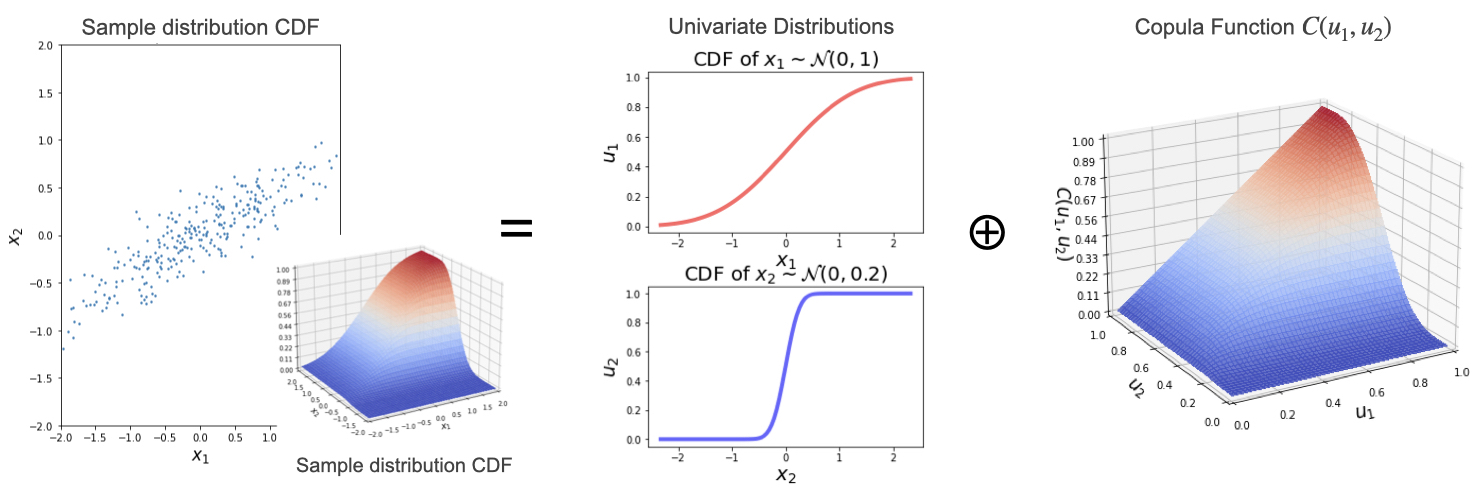
\includegraphics[width=\linewidth]{copula/figs/copula.jpeg}
    \caption{An example copula, where we express a multivarite Gaussian with correlation $\rho = 0.8$ with two univariate distributions and a Copula function $C(u_1, u_2)$.} 
    \label{fig:copula}
\end{figure}
